\chapter{Proposed Methodology}
\label{ch:method}

\section{Overview}

The methodology has four strands (Figure~\ref{fig:methodflow}). Each stage is trained on the dataset
that carries its label, with leakage controlled at the radiograph level. A theory of the tooth-level
score supplies an image-blind baseline in closed form. Every comparison is paired on the same images
and reported with cluster-bootstrap intervals, per cohort and per site. Any change to a default
checkpoint must pass a rule written before the evidence.

\begin{figure}[!htbp]
\centering
% Methodology workflow. Traced to: data roles (Table 8.1), leakage control (MD5 exclusion, pHash check,
% radiograph-level splits), training recipes (Table 8.4), the constant (eq. 8.2-8.3), evaluation protocol
% (Section 8.7), pre-registration (ef3f453).
\begin{tikzpicture}[node distance=5mm and 6mm]
\node[io,text width=27mm] (d) {Public datasets\\[-1pt]{\normalfont each with one role}};
\node[stage,text width=29mm,right=of d] (l) {Leakage control\\[-1pt]{\normalfont MD5, pHash, split by radiograph}};
\node[stage,text width=27mm,right=of l] (t) {Train each stage\\[-1pt]{\normalfont recorded recipe, seed 42}};
\node[stage,text width=27mm,right=of t] (v) {Select on validation\\[-1pt]{\normalfont never on a test set}};
\node[cari,text width=29mm,below=9mm of d] (c) {Image-blind constant\\[-1pt]{\normalfont fitted off the test set}};
\node[cari,text width=29mm,right=of c] (e) {Paired evaluation\\[-1pt]{\normalfont per cohort, per site}};
\node[cari,text width=27mm,right=of e] (s) {Intervals\\[-1pt]{\normalfont cluster bootstrap, DL + HKSJ}};
\node[filt,text width=27mm,right=of s] (r) {Pre-registered rule\\[-1pt]{\normalfont committed before training}};
\node[rept,text width=40mm,below=9mm of r] (a) {Adopt, or keep as ablation;\\report both};
\draw[arr] (d) -- (l); \draw[arr] (l) -- (t); \draw[arr] (t) -- (v);
\draw[arr] (v.south) -- ++(0,-3mm) -| (e.north);
\draw[arr] (c) -- (e); \draw[arr] (e) -- (s); \draw[arr] (s) -- (r); \draw[arr] (r) -- (a);
\node[soft=p2maroon,text width=35mm,below=9mm of e] (lock) {Ningxia locked: test only, never tuned on};
\draw[darr] (lock) -- (e);
\end{tikzpicture}

\caption[Methodology workflow]{Methodology workflow, from data to an adopted checkpoint.}
\label{fig:methodflow}
\end{figure}

\section{Datasets and Task Allocation}

No single public dataset provides every label needed for tooth detection, numbering, caries and an
abnormality flag in one consistent format, so each dataset has a strict role
(Table~\ref{tab:datasets}). Labels are not mixed across tasks unless a direct spatial mapping exists.

\begin{table}[!htbp]
\centering
\caption[Datasets and their roles]{Datasets and their roles. Updated from Table 4.1 of the Phase 2 report.}
\label{tab:datasets}
\small
\begin{tabularx}{\textwidth}{@{}L{2.7cm}L{3.3cm}YL{2.8cm}@{}}
\toprule
Dataset & Annotation & Role in Phase 3 & Licence\\
\midrule
DENTEX~\cite{hamamci2023dentex} & Quadrant, enumeration and diagnosis boxes & Detector and numbering training; caries severity and the retained crop classifier; the development evaluation cohort (164 images) & CC BY-NC-SA 4.0\\
Tufts~\cite{panetta2022tufts} & 1,000 OPGs; tooth boxes, expert text, abnormality masks & Detector and numbering training; the abnormality flag; a held-out numbering test split (143 images) & Not redistributable\\
CariesXrays~\cite{chen2024cariesxrays} & 6,000 OPGs; lesion boxes & Lesion-detector training (4,800) and validation (1,200) & Used under citation\\
Kaggle dual-labelled & Tooth boxes and numbers & Third corpus of the detector & Kaggle release terms\\
Ningxia~\cite{li2024multicenter} & Lesion annotations; four test sites & External caries evaluation only (337 images); never trained or tuned on & Public release, no formal licence\\
UFBA-425~\cite{budagam2024oralbbnet} & Tooth annotations & External numbering evaluation only (425 images) & Public release\\
\bottomrule
\end{tabularx}
\end{table}

For the Tufts branch, only radiographs with all three sources present (tooth boxes, expert text and
masks) were kept after the join. This left a working pool of 423 OPGs, from which the Phase 2 work
built 22,806 tooth-level crops with a strong imbalance, about 96\% normal and 4\% abnormal, a ratio of
23.84 to 1 (Figure~\ref{fig:tuftscoverage}). % {C080}

\begin{figure}[!htbp]
\centering
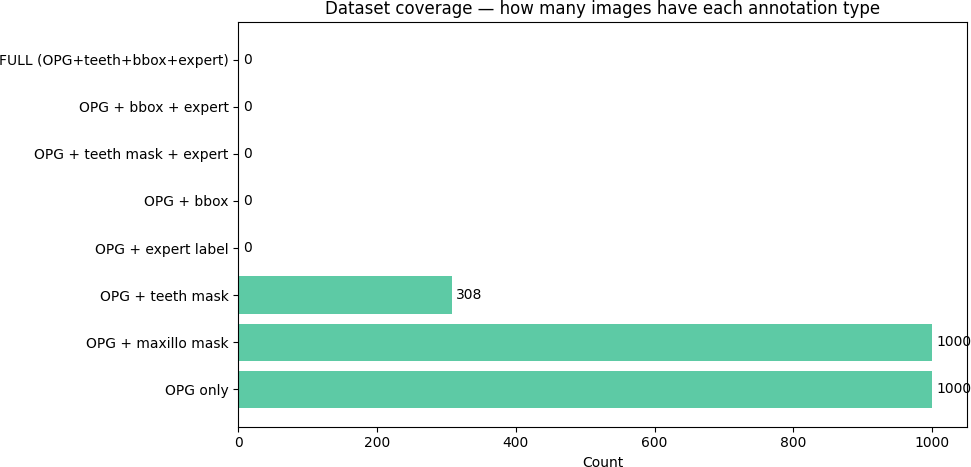
\includegraphics[width=0.66\textwidth]{figures/phase2/p2_4_01_tufts_coverage.png}
\caption[Tufts annotation coverage]{Coverage matrix used to identify the Tufts radiographs that carry
all required annotations (Phase 2 report, Figure 4.1).}
\label{fig:tuftscoverage}
\end{figure}

\section{Evaluation Cohorts}

Table~\ref{tab:cohorts} lists the evaluation populations. All splits are made by image. DENTEX's
disease subset has 250 annotated OPGs; MD5 hashing found 86 of them byte-identical to images the
models trained on (85 in numbering, 1 in detection), leaving 164 scored, of which 148 carry a caries
lesion (479 lesions on 477 teeth). The Ningxia release divides its test data into four sets: test2
comes from the dataset's training centre, and test1, test3 and test4 are described as cross-centre.
These are treated as four sites. % {C060}

\begin{table}[!htbp]
\centering
\caption[Evaluation cohorts]{Evaluation cohorts, units and exposure. Each row is a separate analysis
population; counts are not summed across rows.}
\label{tab:cohorts}
\small
\begin{tabularx}{\textwidth}{@{}L{2.8cm}L{1.4cm}L{4.3cm}Y@{}}
\toprule
Cohort & Images & Unit (n) & Role and exposure\\
\midrule
DENTEX disease & 164 & 936 teeth; 477 carious; 479 lesions & development; the detector trained on other DENTEX images\\
Ningxia, 4 sites & 337 & 1,013 lesions & external; never trained on; informed the lesion detector's adoption\\
CariesXrays & 1,200 & 2,815 lesions & external, except to the lesion detector (its validation split)\\
Tufts test & 143 & 3,760 / 3,892 teeth & numbering / Stage 4 (182 labelled); both trained on Tufts training images\\
UFBA-425 & 425 & 11,591 teeth & numbering; no model trained on it\\
\bottomrule
\end{tabularx}
\end{table}

\section{Data Preparation and Leakage Control}

\subsection{Leakage Control}

\begin{itemize}
\item \textbf{Exact duplicates.} Every evaluation image is hashed (MD5) against every training image;
  the 86 byte-identical DENTEX images are excluded from scoring.
\item \textbf{Near duplicates.} A perceptual-hash search (pHash and dHash) of the 164 scored DENTEX
  images against the 1,389 other DENTEX images checks for re-encoded or resized copies
  (Section~\ref{sec:res-controls}).
\item \textbf{Radiograph-level splits.} Training, validation and test sets are split by radiograph, so
  no radiograph contributes crops to two sets. The Tufts split is frozen and regenerated from code.
\item \textbf{Locked external data.} Ningxia is used only for testing and never for training,
  threshold choice or checkpoint selection.
\end{itemize}

\subsection{Preprocessing Retained from Phase 2}

\textbf{Bounding-box correction.} The raw Tufts annotation stores corners as $[y_1, x_1, y_2, x_2]$,
not $[x, y, w, h]$. Each box is converted with $x = x_1$, $y = y_1$, $w = x_2 - x_1$ and $h = y_2 - y_1$.
Without this correction every crop would have been cut from the wrong place.

\textbf{Asymmetric expanded crop.} For the abnormality flag each tooth box is expanded 1.5 times in
width and 2.0 times in height, clipped to the image and resized to 224 by 224. Teeth on a panoramic
radiograph are much taller than they are wide, so a symmetric expansion would take in neighbouring
teeth while still missing bone below the root.

\textbf{Overlap-ratio labelling.} Intersection over union was rejected for labelling crops, because the
expert masks are sparse and even a genuinely positive crop has an IoU near zero. The label uses the
share of mask pixels inside the crop,
\begin{equation}
\text{overlap} = \frac{\text{non-zero mask pixels inside the crop}}{\text{crop area}},
\label{eq:overlap}
\end{equation}
with a threshold of 0.01 chosen by inspecting the distribution of overlaps
(Figure~\ref{fig:overlapdist}).

\begin{figure}[!htbp]
\centering
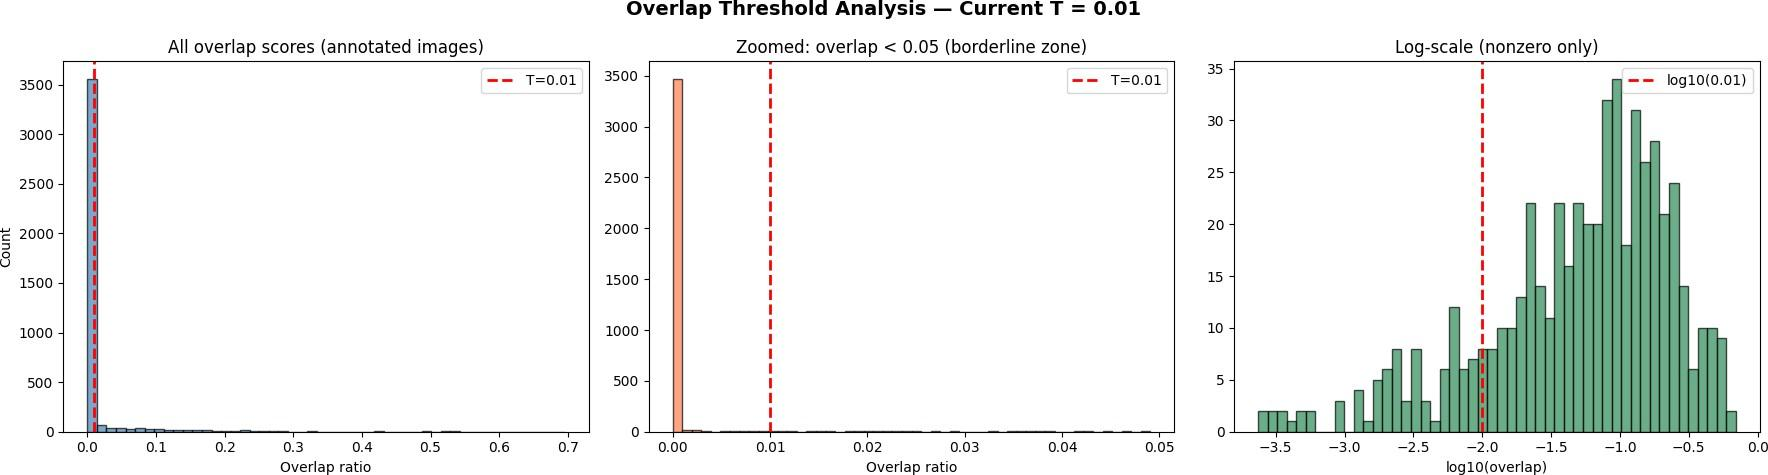
\includegraphics[width=0.8\textwidth]{figures/phase2/p2_4_02_overlap_distribution.jpg}
\caption[Distribution of overlap ratios]{Distribution of overlap ratios used for tooth-level label
assignment (Phase 2 report, Figure 4.2).}
\label{fig:overlapdist}
\end{figure}

\textbf{Box jitter.} A random perturbation of $\pm$15\% is applied to the Tufts boxes during crop
generation, to simulate the localisation noise of a detector and make the classifier less sensitive to
small misalignments. % {C082}

\textbf{CLAHE for the CEJ heuristic.} The exploratory CEJ branch enhanced each crop with
contrast-limited adaptive histogram equalisation (clip limit 2.0, 8 by 8 tiles) and light Gaussian
smoothing; this path is not used by the classifiers.

\textbf{Class imbalance (Phase 2 model).} For the Phase 2 binary model the normal class was
undersampled from 17,473 training crops to 2,500, and the 237 abnormal crops were expanded to 711 by
offline augmentation (random horizontal flip, rotation within 10\textdegree, brightness and contrast
jitter, and a small translation), giving the counts in Table~\ref{tab:p2data}.

\begin{table}[!htbp]
\centering
\caption[Tufts data summary of the Phase 2 binary model]{Tufts data summary of the Phase 2 binary model
(Phase 2 report, Table 4.2). Phase 3 found that this validation split shared radiographs with the
training split (Section~\ref{sec:res-stage4}).}
\label{tab:p2data}
\small
\begin{tabular}{@{}lrrr@{}}
\toprule
Split / subset & Normal & Abnormal & Total\\
\midrule
Raw training crops & 17,473 & 237 & 17,710\\
Resampled training crops & 2,500 & 711 & 3,211\\
Validation crops & 1,499 & 59 & 1,558\\
\bottomrule
\end{tabular}
\end{table}

The Phase 2 report stated that this split was made at the OPG level. The Phase 3 audit found the
opposite: it was a crop-level split, and every one of its validation radiographs also supplied
training crops. That is why the Phase 2 validation figure did not survive a held-out test
(Section~\ref{sec:res-stage4}), and why the Phase 3 model was retrained by radiograph.

\section{Model Training}

All classifier heads are ResNet18 networks pre-trained on ImageNet, with the final layer replaced; the
two detectors are YOLOv11l. Table~\ref{tab:training} gives each shipped model's recipe. Every model
was selected on its own validation split and is a single training run, except Stage~4a, which was
trained with three seeds.

\begin{table}[!htbp]
\centering
\caption[Training recipes of the shipped models]{Training recipes of the shipped models, from each
checkpoint's \texttt{run\_summary.txt}.}
\label{tab:training}
\footnotesize
\begin{tabularx}{\textwidth}{@{}L{2.4cm}L{3.4cm}YL{2.0cm}@{}}
\toprule
Model & Data & Recipe & Kept checkpoint\\
\midrule
Stage 1 detector, YOLOv11l & Tufts + DENTEX + Kaggle, balanced per corpus & 1,024 px, batch 32, AdamW, lr 0.001 with cosine decay, up to 150 epochs (patience 30), mosaic and vertical flip off, seed 42 & best on Tufts validation\\
Stage 2 head, ResNet18 + 4 features & DENTEX + Tufts crops, $1.5\times$ & 224 px, batch 64, lr 0.001 (backbone $\times$0.1), 15 epochs, seed 42 & epoch 12\\
Stage 3a lesion detector, YOLOv11l & 4,800 CariesXrays + 650 DENTEX images (replicated), 9,600 samples per epoch & one class, batch 16, up to 120 epochs (patience 25), mosaic and vertical flip off & epoch 29 of 54\\
Stage 3a crop classifier, ResNet18 & 6,616 tight crops from 260 DENTEX images & 15 epochs, augmented, class weights 3.2849 / 0.5898, seed 42 & epoch 15\\
Stage 3b severity, ResNet18 & DENTEX caries crops & cross-entropy with class weights; Adam, lr 0.001 on the final layer then $3\times10^{-5}$ on the whole network & Phase 2 bundle\\
Stage 4a flag, ResNet18 & 678 Tufts radiographs (36,360 crops) & focal loss ($\gamma$ = 2), Adam lr $10^{-4}$, weight decay $10^{-4}$, batch 32, up to 50 epochs (stop after 10 without gain) & epoch 16 of 26 (seed 42)\\
\bottomrule
\end{tabularx}
\end{table}

Mosaic augmentation and vertical flips are disabled for both detectors by a house rule: a mosaic
breaks the spatial context of a panoramic image, and a vertical flip swaps the upper and lower arches.
Training ran on cloud GPUs and on a laptop accelerator; inference needs neither. % {C083}

\section{The Image-Blind Constant}
\label{sec:method-constant}

\subsection{F1 of a Constant in Closed Form}

Let $N$ images be scored, $P$ be the number of carious teeth over all of them, and $n_c$ the number of
images in which tooth code $c$ is carious, so that $p_c = n_c/N$ is the prevalence of caries at
position $c$. A constant answers the same set $S$ of codes for every image. Its true positives are
$\sum_{c \in S} n_c$ and it names $|S|\,N$ codes, so its micro-averaged F1 is
\begin{equation}
F_1(S) = \frac{2 \sum_{c \in S} n_c}{|S|\,N + P}.
\label{eq:constf1}
\end{equation}
The equation counts every named code as a prediction, present tooth or not, as the scorer does, and
it applies to any set prediction scored by micro-F1 over a fixed label set. Nothing in it depends on an
image. The constant's recall, $\sum_{c \in S} n_c / P$, is the share of carious teeth that lie at its
codes.

\subsection{The Selection Rule}

Write $A = \sum_{c \in S} n_c$ and $k = |S|$. Adding a code $c \notin S$ raises the score,
$2(A+n_c)/((k+1)N+P) > 2A/(kN+P)$, if and only if
\begin{equation}
p_c > \tfrac{1}{2}\, F_1(S).
\label{eq:rule}
\end{equation}
For any fixed size the best set is the $k$ most prevalent codes, so the F1-optimal constant is a
prefix of the codes sorted by prevalence. Writing $S_k$ for the $k$ most prevalent codes, F1 rises
along $S_1, S_2, \dots$ to a single peak: if code $k+1$ fails~\eqref{eq:rule} against $S_k$, then
$p_{k+1} \le \tfrac{1}{2}F_1(S_{k+1})$ as well, so every later, less prevalent code fails too. The
optimum is the prefix cut where~\eqref{eq:rule} first fails, and it holds exactly the codes with
$p_c > \tfrac{1}{2}F_1^{*}$: a functional of the caries prior alone. That first molars are the most
caries-susceptible teeth is long established in caries epidemiology~\cite{batchelor2004grouping}; the
prior, and with it the floor, depends on the population's age and exposure. % {C010}

The constant is fitted on the 78 DENTEX images that were excluded from scoring because the models
trained on them, and frozen before it is scored (Figure~\ref{fig:prior}). % {C010}

\begin{figure}[!htbp]
\centering
\includegraphics[width=0.94\textwidth]{figures/repo/R05_positional_prior.pdf}
\caption[The positional prior and the constant it implies]{The positional prior and the constant it
implies. (a) Share of images in which the expert marked each FDI code carious, in chart order
(patient's right to left, as displayed): grey, the fit set (78 DENTEX images with caries, excluded from
scoring because the models trained on them); orange, the 164 scored images. Magenta: the eight codes
rule~\eqref{eq:rule} admits; dashed: the final threshold $F_1/2 = 0.196$. (b) F1 of the $k$ most
prevalent fit-set codes.}
\label{fig:prior}
\end{figure}

\subsection{Lesion Agreement and the Cohort's Prior}

The second metric family scores lesions rather than codes. Let a cohort contain $L$ expert lesions,
let $T(\ell)$ be the detected tooth that contains lesion $\ell$, and let $\mathcal{F}$ be the set of
teeth a system flags. Lesion agreement is
\begin{equation}
A(\mathcal{F}) = \frac{1}{L} \sum_{\ell} \mathbf{1}\big[\, T(\ell) \in \mathcal{F} \,\big].
\label{eq:agreement}
\end{equation}
It has no negative class, so it can only rise as $\mathcal{F}$ grows, and flagging every detected tooth
reaches its ceiling, the share of lesions inside any detected tooth; it must be read beside the number
of teeth flagged. For the constant, $\mathcal{F}$ is the eight molar boxes the front end finds, so $A$
is the cohort's prior mass on those molars. That prior mass varies between cohorts and between sites
of one cohort, as Zech et al.\ found for pneumonia prevalence between hospitals~\cite{zech2018variable},
so systems can be compared only when paired on the same images, cohort by cohort and site by site.

\section{A Test for a Positional Shortcut}

If a per-tooth classifier has learned the probability of caries given position, and not only given
pixels, two consequences follow. Its score on truly healthy teeth should rise with the base rate of
their position, because the prior lifts every tooth of a caries-prone type. And its ranking should
survive only partly when position is held fixed: the within-type area under the ROC curve (AUC), which
ranks carious against healthy teeth of the same type, removes the positional cue and keeps the image
signal. Both tests are applied to the crop classifier on 863 held-out tooth crops from 34 radiographs,
cut with ground-truth boxes so that the front end plays no part (Section~\ref{sec:res-shortcut}).

A whole-image lesion detector receives no tooth identity: to flag a tooth it must place a box mostly
inside it. It can express a positional prior only by drawing boxes over molars where it sees no lesion,
and each such box costs precision under~\eqref{eq:constf1} and earns agreement
under~\eqref{eq:agreement} only if a lesion happens to lie there. If the detector's lead over the
constant comes from reading the image, it should therefore come with fewer flagged teeth, and within
each tooth type its flags should be carious more often than the classifier's. % {C093}

\section{Evaluation Protocol}
\label{sec:method-eval}

\subsection{Systems Compared}

Four systems answer one question, which teeth in this radiograph show caries, on the same 164 images:
the pipeline (with each Stage-3a method), Qwen2.5-VL-32B (33.45\,B parameters) and Qwen2.5-VL-7B
(8.29\,B), both zero-shot with the FDI scheme in the prompt and also shown a blank grey and a
random-noise image as content-free controls, and the image-blind constant.

\subsection{Metrics}

FDI-set F1~\eqref{eq:constf1} is micro-averaged over teeth. Lesion agreement~\eqref{eq:agreement}
matches each expert lesion to a flagged tooth. On DENTEX it uses a greedy intersection over union of at
least 0.30 with a centroid fallback. On the external cohorts it uses centroid containment, because their
lesions are small (median 731 pixels) inside tooth boxes of about 25,000 pixels, so every comparison is
made within a cohort. % {C094}

\subsection{Statistics}

Teeth within one radiograph share exposure, anatomy and annotator, so their errors are correlated. All
intervals are 95\% percentile bootstrap confidence intervals (CI) over images, not teeth, the cluster bootstrap that stays
consistent when clusters carry random effects~\cite{field2007bootstrapping}. Unless stated, 10,000
resamples with seed 42 are used; the crop classifier's calibration average precision (AP) uses 2,000, its within-type AUC
5,000, and the two abstention gains 1,000 with seed 0. For two systems scored on the same images, the
paired difference is recomputed on every resample, and its 2.5th and 97.5th percentiles give the
interval. Differences are system minus comparator in percentage points (pp). % {C095}

Across the four Ningxia sites, the per-site differences $\Delta_j$ with variances $v_j$ (from each
site's interval width) are pooled by DerSimonian--Laird random effects~\cite{dersimonian1986meta},
\begin{equation}
\hat\mu = \frac{\sum_j \Delta_j / (v_j + \hat\tau^2)}{\sum_j 1 / (v_j + \hat\tau^2)},
\label{eq:dl}
\end{equation}
where the between-site variance $\hat\tau^2$ is estimated from Cochran's $Q$, and
$I^2 = (Q - k + 1)/Q$ is the share of variation due to sites~\cite{higgins2002quantifying}. A fixed-site
interval asks whether a system led at these sites; the random-effects prediction interval asks whether
it would lead at another~\cite{riley2011interpretation}. With only four sites the DerSimonian--Laird
interval is too narrow, so the Hartung--Knapp--Sidik--Jonkman (HKSJ) interval~\cite{inthout2014hartung}
and a Q-profile interval for $\tau$~\cite{viechtbauer2007confidence} are reported beside it.

\subsection{Matched-Volume Comparison}

A system that names more teeth than the constant can buy F1 with volume. Each system is therefore also
compared with an image-blind answer that names exactly as many codes: the $k$ most prevalent fit-set
codes on some images and the $k+1$ most prevalent on the rest, a mixture chosen without looking at any
image, whose true positives and named codes are linear in the mixing fraction.

\subsection{Estimation, Not Testing}

Results are reported as estimates with intervals, not as a family of hypothesis tests, so no
multiplicity correction is applied across cohorts, arms, metrics and sites. The theory of
Section~\ref{sec:method-constant} was formulated after the measurements it is checked against, so its
check in Chapter~\ref{ch:results} is a consistency check, not a test of predictions made in advance.

\section{Pre-Registration and Experiment Governance}
\label{sec:method-prereg}

Changes to a default checkpoint were proposed as numbered ``levers'', each with an acceptance rule
committed before the arm was trained (Table~\ref{tab:levers}, Figure~\ref{fig:levers}). The caries
reformulation's rule, committed as \texttt{ef3f453} before any arm was trained, required the lesion
detector to beat both the image-blind constant and the crop classifier on at least two of three
cohorts, with the interval excluding zero, at no more than 1.5 times their rate of flagged teeth.
Because Ningxia was one of the three cohorts, it informed the adoption, and the lead measured on it is
optimistic by construction. % {C021}

\begin{table}[!htbp]
\centering
\caption[Levers attempted and their outcomes]{Levers attempted and their outcomes.}
\label{tab:levers}
\small
\begin{tabularx}{\textwidth}{@{}L{1.0cm}L{4.4cm}Y@{}}
\toprule
Lever & Change & Outcome\\
\midrule
1 & Multi-corpus detector (Tufts + DENTEX) & DENTEX numbering rose sharply; the Tufts guard failed: kept as an ablation\\
2 & Stand-alone CariesXrays lesion detector & Level with the benchmark's own method; a benchmark row, not a pipeline component\\
A & Multi-corpus detector, three- and four-corpus arms, balanced per corpus & Primary metric and external-caries guard passed; the Tufts box mAP guard failed: an ablation, the three-corpus arm later made the default by a separate decision\\
A2 & Frozen-backbone Tufts fine-tune of Lever A & Tufts test guard still failed: an ablation\\
B & Caries as whole-image lesion detection & Met the rule on two of three cohorts: \textbf{adopted}\\
C & Structural FDI post-processing & Null: not adopted\\
\bottomrule
\end{tabularx}
\end{table}

\begin{figure}[!htbp]
\centering
% Experiment lineage. Traced to transfer.md section 2.6 (levers 1, 2, A, A2, B, C) and models/README.md.
\begin{tikzpicture}[node distance=5mm and 7mm,
  lev/.style={box,fill=#1,text width=32mm,minimum height=10mm,font=\sffamily\tiny\bfseries}]
\node[io,text width=32mm] (base) {Phase 2 modules\\[-1pt]{\normalfont crop classifier, Tufts-only detector}};
\node[lev=p2arrow,right=of base,yshift=13mm] (l1) {Lever 1: multi-corpus detector\\[-1pt]{\normalfont Tufts guard failed}};
\node[lev=p2orange,right=of l1] (la) {Lever A: 3- and 4-corpus detector\\[-1pt]{\normalfont arm 3C made default, 11 Oct}};
\node[lev=p2arrow,right=of la] (la2) {Lever A2: frozen fine-tune\\[-1pt]{\normalfont Tufts guard failed}};
\node[lev=p2arrow,right=of base,yshift=-1mm] (l2) {Lever 2: CariesXrays detector\\[-1pt]{\normalfont benchmark row}};
\node[lev=p2green,right=of l2] (lb) {Lever B: lesion detector\\[-1pt]{\normalfont adopted 4 Sep, 2 of 3 cohorts}};
\node[lev=p2arrow,right=of base,yshift=-15mm] (rep) {Five crop-classifier repairs\\[-1pt]{\normalfont none separated from zero}};
\node[lev=p2arrow,right=of rep] (lc) {Lever C: FDI structural repair\\[-1pt]{\normalfont null}};
\node[lev=p2green,right=of lc] (s4) {Stage 4a by radiograph\\[-1pt]{\normalfont default 13 Oct}};
\draw[arr] (base.east) -- ++(2mm,0) |- (l1.west); \draw[arr] (l1) -- (la); \draw[arr] (la) -- (la2);
\draw[arr] (base.east) -- ++(2mm,0) |- (l2.west); \draw[arr] (l2) -- node[lbl,above]{same arch.} (lb);
\draw[arr] (base.east) -- ++(2mm,0) |- (rep.west); \draw[arr] (rep) -- (lc);
\draw[darr] (rep.north) -- node[lbl,right]{task changed} (lb.south west);
\end{tikzpicture}

\caption[Experiment lineage]{Experiment lineage. Green: adopted into the pipeline; grey: ablation or
null; orange: adopted by a separate decision against a failed guard.}
\label{fig:levers}
\end{figure}
